% !TeX spellcheck = de_CH_frami

\section{MOS-Transistoren (Kap. 5)}

\begin{minipage}[c]{0.54\textwidth}
	\textbf{Bulk-Anschluss}\\
	Wenn der Bulk-Anschluss nicht gezeichnet ist, gilt die Konvention, dass der Bulk des n-Transistors immer mit VSS und derjenige des p-Transistors immer mit VDD verbunden ist.
	\subsection{Bestimmung des Arbeitsbereichs}
	1. Bestimmung ob weak, moderate oder strong inversion.\\
	2. Berechnen der Sättigungsspannung.\\
	3. Wenn $\mid V_{DS}\mid > \mid V_{DS,sat}\mid$ = gesättigt
\end{minipage}
\begin{minipage}[c]{0.13\textwidth}
	\uline{\textbf{NMOS:}}\\
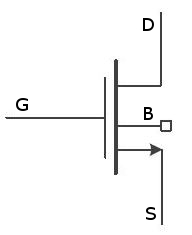
\includegraphics[width=1\textwidth]{chapters/Transistoren/images/N-MOS}
\end{minipage}
\begin{minipage}[c]{0.13\textwidth}
	\uline{\textbf{PMOS:}}\\
	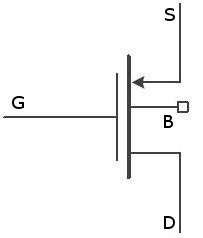
\includegraphics[width=1\textwidth]{chapters/Transistoren/images/P-MOS}
\end{minipage}
\begin{minipage}[c]{0.2\textwidth}
	\textbf{Legende:}\\
	G: Gate\\
	D: Drain\\
	S: Source\\
	B: Bulk
\end{minipage}
\\[2ex]
\begin{minipage}[c]{0.76\textwidth}
	\begin{tabular}{|l|l|l|}
		\hline
		\textbf{Arbeitsbereich}& \textbf{Bedingung} & \textbf{Sättigungspannung}\\ \hline
		weak inversion& $0 < V_{GS} < V_T - \SI{60}{\milli\volt}$ & $V_{DS,sat}\approx 5\Phi _t \approx \SI{130}{\milli\volt}$ \\
		& &(bei $T = \SI{300}{\kelvin} = \SI{27}{\degreeCelsius}$) \\
		$I'_D < I'_M$& & $V_{GS} = V_M +n_M \cdot \Phi_t \cdot \ln{\frac{I_D}{\frac{W}{L}\cdot I_M}}$\\ \hline
		moderate inversion& $V_T - \SI{60}{\milli\volt} < V_{GS} < V_T + \SI{160}{\milli\volt} $ & \\
		$I'_M < I'_D < I'_H$& & \\ \hline
		strong inversion& $V_T + \SI{160}{\milli\volt} < V_{GS}$ & $V_{DS,sat} = V_{GS}-V_T = \sqrt{\frac{2I_D}{\beta}}$\\
		$I'_H < I'_D$& & \\ \hline
	\end{tabular}
\end{minipage}
\begin{minipage}[c]{0.24\textwidth}
	\uline{\textbf{Formeln:}}\\
	$I_D = \frac{W}{L}\cdot I'_D$\\
	$\Phi_t = V_{temp} = \frac{k\cdot T}{e}$\\
	$\Phi_t = \SI{25.9}{\milli\volt}$ @ $T = \SI{27}{\degreeCelsius}$\\
	$\beta = \frac{W}{L} \cdot \beta_0$ \\[2ex]
	\uline{\textbf{Konstanten:}}\\
	$k = \SI{1.38e-23}{\joule /\kelvin}$\\
	$e = \SI{1.60e-19}{\coulomb}$
\end{minipage}

\subsection{Kennlinien}
\subsubsection{Ausgangskennlinie}

\begin{minipage}[c]{0.35\textwidth}
	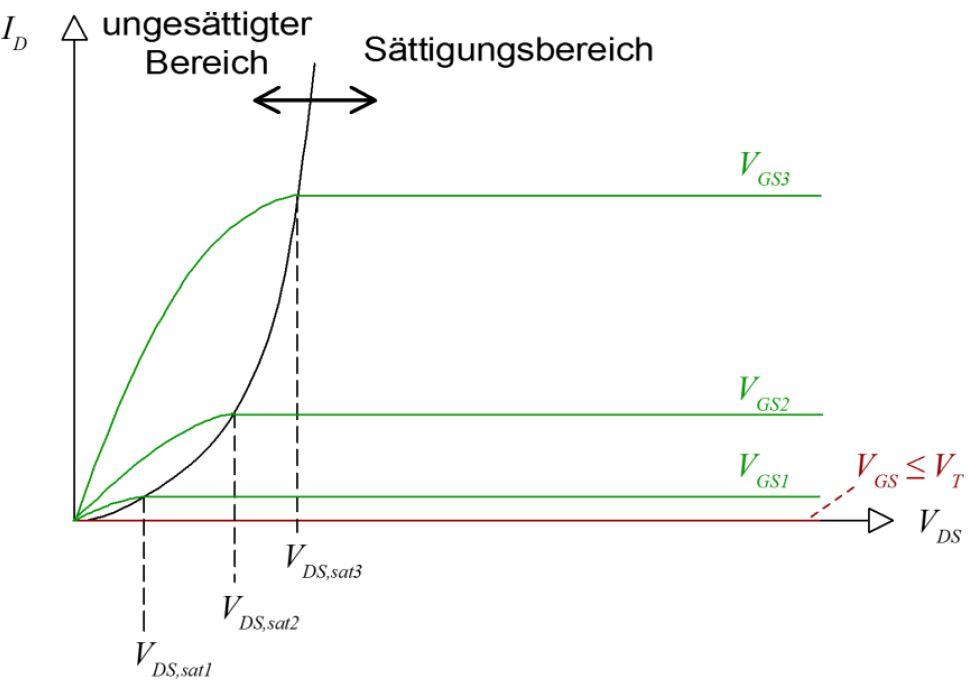
\includegraphics[width=1\linewidth]{chapters/Transistoren/images/Ausgangskennlinie}
\end{minipage}
\begin{minipage}[c]{0.65\textwidth}
	\textbf{Gesättigt}, Stromquellen-Betrieb:\\
	Geraden horizontal, dann ist $r_{DS} = \infty$ (idealer Transistor).\\
	Anstieg der Geraden entspricht Ausgangsleitwert $g_o$ o. Ausgangswiderstand $r_{DS}$\\
	$r_{DS} = \frac{1}{g_o} = \frac{dV_{DS}}{dI_D} \approx \frac{\Delta V_{DS}}{\Delta I_D}$\\ \\
	\textbf{Ungesättigt}, Widerstandsbetrieb:\\
	Je steiler die Gerade, desto kleiner $r_{DS}$
\end{minipage}

\subsubsection{Transferkennlinie}
\begin{minipage}{0.4\textwidth}
	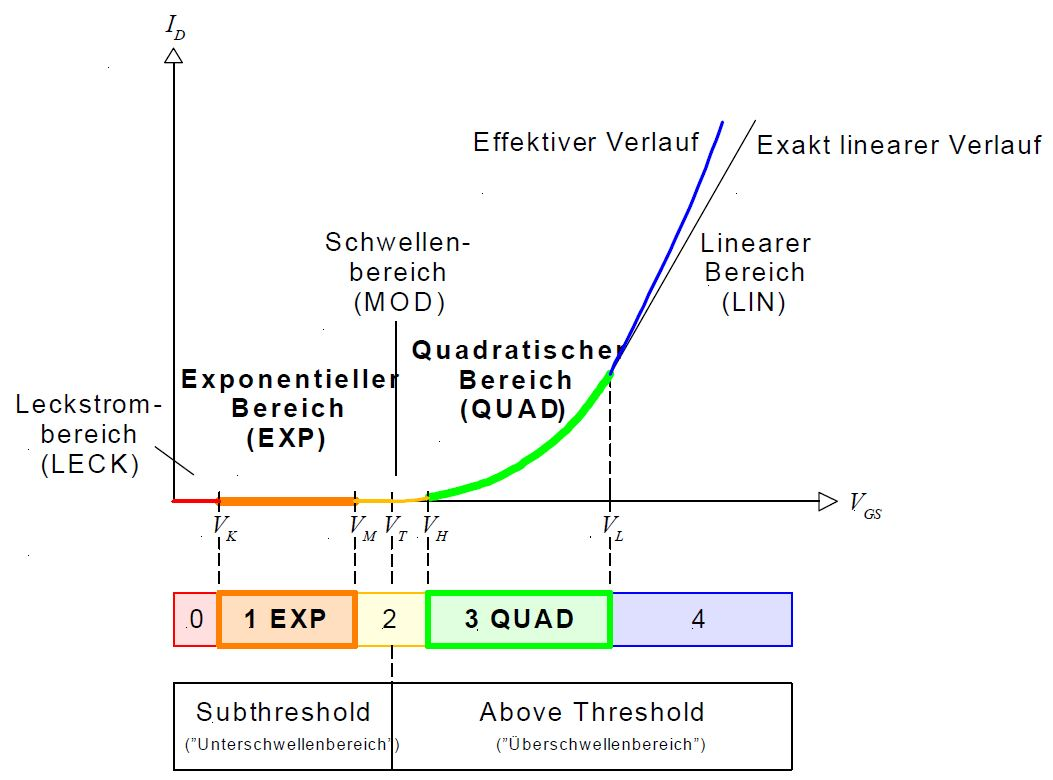
\includegraphics[width=1\linewidth]{chapters/Transistoren/images/Transferkennlinie}
\end{minipage}
\begin{minipage}{0.6\textwidth}
	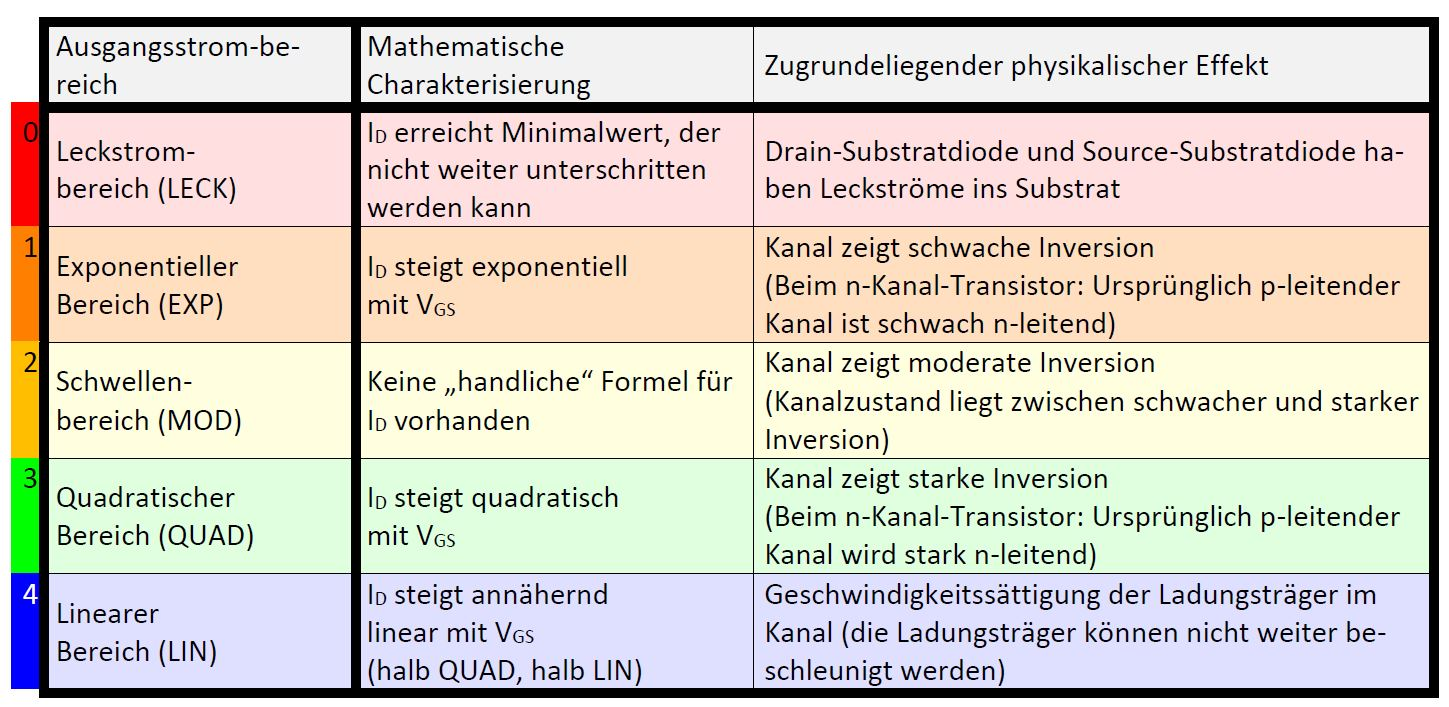
\includegraphics[width=1\linewidth]{chapters/Transistoren/images/Ausgangsstrombereich} 
\end{minipage}

\subsection{Drainstromgleichungen}
\begin{tabular}{|l|l|l|}
	\hline
	\textbf{Ausgangsstrom} & \multicolumn{2}{c|}{\textbf{Ausgangsspannungsbereich} ($V_{DS}$-Bereich)}\\
	($I_D$-,$V_{GS}$-Bereich)&Transistor ungesättigt ($\vert V_{DS}\vert < \vert V_{DS,sat}\vert$)&Transistor gesättigt ($\vert V_{DS} \vert \geq \vert V_{DS,sat} \vert$)\\ \hline
	EXP-Bereich (n-Kanal)&$I_D = I_M e^{\frac{V_{GS}-V_M}{n_M \Phi_t}}(1-e^{\frac{-V_{DS}}{\Phi_t}})\textcolor{gray}{(1 + \lambda V_{DS})}$&$I_D=I_M e^{\frac{V_{GS}-V_M}{n_M \Phi_t}}\textcolor{gray}{(1+\lambda V_{DS})}$\\ \hline
	QUAD-Bereich (n-Kanal)&$I_D=B[(V_{GS}-V_T)V_{DS}-\frac{{V_{DS}}^2}{2}]\textcolor{gray}{(1+\lambda V_{DS})}$&$I_D=\frac{\beta}{2}(V_{GS}-V_T)^2 \textcolor{gray}{(1+\lambda V_{DS})}$\\ \hline
	EXP-Bereich (p-Kanal)&$I_D = I_M e^{-\frac{V_{GS}-V_M}{n_M \Phi_t}}(1-e^{\frac{-V_{DS}}{\Phi_t}})\textcolor{gray}{(1 - \lambda V_{DS})}$&$I_D=I_M e^{-\frac{V_{GS}-V_M}{n_M \Phi_t}}\textcolor{gray}{(1-\lambda V_{DS})}$\\ \hline
	QUAD-Bereich (p-Kanal)&$I_D=-B[(V_{GS}-V_T)V_{DS}-\frac{{V_{DS}}^2}{2}]\textcolor{gray}{(1-\lambda V_{DS})}$&$I_D=-\frac{\beta}{2}(V_{GS}-V_T)^2 \textcolor{gray}{(1-\lambda V_{DS})}$\\
	\hline
\end{tabular}\\ \\
Wird die Kanallängenmodulation vernachlässigt, kann einfach der \textcolor{gray}{$(1 \pm\lambda V_{DS})$} Term weggelassen werden.

\subsection{Parameter}
\begin{tabular}{|p{0.05\textwidth}|p{0.21\textwidth}|p{0.64\textwidth}|}
	\hline
	$V_{DS,sat}$&Sättigungsspannung&im EXP-Bereich:   $V_{DS,sat} = -5\Phi_t$ \\ 
	&&im QUAD-Bereich:	$V_{DS,sat} = V_{GS}-V_T$\\ \hline
	$V_T$&Schwellenspannung&Typisch \SI{0.6}{\volt} beim n-Kanal, resp. \SI{-0.6}{\volt} beim p-Kanal.\\
	&& $V_T$ ist stark von der Source-Bulk-Spannung abhängig (Body-Effekt):\\
	&&$V_T = V_{T0}\pm \Delta V_T$ mit $\Delta V_T = \lambda \left( \sqrt{V_{SB} \pm \Phi_0} - \sqrt{\Phi_0}\right)$\\
	&&(+ für n-Kanal-Transistoren, - für p-Kanal Transistoren)\\
	&& $\gamma_N \approx 0.6 \sqrt{V}$ bzw. $\gamma_P \approx 0 \sqrt{V}$ ($\sqrt{V}$ ist die Einheit von $\gamma$)\\
	&&Handrechnung: $\gamma \approx \gamma_N \approx \gamma_P \approx 0.6\sqrt{V}$\\ \hline
	$\Phi_t$&Temperaturspannung&$\Phi_t = V_{Temp} = \frac{kT}{e} = \SI{86.2}{\micro\volt / \kelvin} \cdot T$\\
	&&somit ist $\Phi_t = \SI{25.9}{\milli\volt}$ bei $T=\SI{300}{\kelvin}$ bzw. $\SI{27}{\degreeCelsius}$\\ \hline
	$I_M$&Drainstrom&Drainstrom an der Grenze zwischen schwacher und moderater Inversion.\\
	&&$I_M=\frac{W}{L}\cdot I'_M$\\
	&&$I'_M$ ist der spezifische Drainstrom an der Grenze\\ \hline
	$n_M$&Unterschwellen-&Der Faktor $n_M$ ist von der Source-Bulk-Spannung $V_{SB}$ abhängig:\\
	&Neigungsfaktor&$n_M=1+\frac{\gamma}{2\sqrt{V_{SB}+\Phi_0}}$\\
	&&mit $\Phi_0 = 2\Phi_F \approx \SI{0.6}{\volt}$. Für $V_{SB} = 0$ erhalten wir $n_M = 1.39$.\\
	&&Häufig wird ein Wert von $n_M \approx 1.5$ angegeben.\\ \hline
	$a_A$&Early-Faktor&\textcolor{gray}{(gemäss Technologieparametern)}\\ \hline
	$V_A$&Early-Spannung&$V_A \approx a_A \cdot L$ \hspace{0.5cm} $V_A$ ist immer positiv\\ \hline
	$\lambda$&Kanallängen-&inverser Wert der Early-Spannung\\
	&Modulationsfaktor&$\lambda = \frac{1}{V_A + V_{DS,sat}} \approx \frac{1}{V_A} \approx \frac{1}{a_AL}$\\	
	&&Bei der Handrechnung wird der MOS-Transistor meistens mit \textcolor{gray}{$\lambda = 0$} idealisiert\\ \hline
	$B$,$\beta$&Transkonduktanz&Steilheit, Verstärkungsfaktor. Dieser Faktor ist im gesättigten ($\beta$) und\\
	&&ungesättigten Bereich ($B$) grundsätzlich verschieden.\\
	&&Es gilt: $\beta=\frac{W}{L}\beta_0$ bzw. $B=\frac{W}{L}B_0$; $B_0\approx \beta_0 = \mu C''_{ox}$ \\ \hline
	$g_m$&Transkonduktanz&Steilheit oder Gate-Steilheit.Beschreibt den Zusammenhang zwischen\\
	&&$I_{DS}$ und $V_{GS}$. Mass für die Verstärkung. \textcolor{gray}{(Siehe Tabelle Kleinsignalparameter)}\\ \hline
	$g_{mb}$&Body-Transkonduktanz&Beschreibt die Wirkung des Body-Effekts. Nur im gesättigtem\\
	&&Stromquellenbetrieb von Bedeutung.\\ 
	&&$g_{mb}=\frac{dI_D}{dV_{SB}}=-g_m(n_M-1)=-g_m(\frac{\gamma}{2\sqrt{V_{SB}+\Phi_0}})$\\ \hline
	$g_0$&Ausgangsleitwert&$g_0=\frac{1}{r_{DS}}=\frac{I_D}{V_A+V_{DS}}$\\ \hline
	$r_{DS}$&Ausgangswiderstand&$r_{DS}=\frac{1}{g_0}\approx\frac{\Delta V_{DS}}{\Delta I_D}$ oder $r_{DS}=\frac{V_A+V_{DS}}{I_{D,real}}\approx\frac{V_A}{I_D}$\\
	&&$V_A$,$V_{DS}$,$I_{D,real}$ immer im Betrag\\ \hline
	$r_{DS0}$&Einschaltwiderstand&Kleinstmöglicher Ausgangswiderstand (bei $V_{DS}=\SI{0}{\volt}$), Widerstandsbetrieb bei $V_{DS}\leq V_{DS,sat}$\\
	&&$r_{DS0}=\frac{dV_{DS}}{dI_D}\vert_{V_{DS}=0} = \frac{1}{\beta(V_{GS}-V_T)}$\\ \hline
	$r_s$&innerer Sourcewiderstand&$r_s=\frac{1}{g_m}=\frac{1}{\sqrt{2\beta I_D}}$\\ 
	\hline
\end{tabular}

\subsection{Kleinsignal-Ersatzschaltungen }
\begin{tabular}{|p{0.21\textwidth}|p{0.21\textwidth}|p{0.19\textwidth}|p{0.25\textwidth}|}
	\hline
	Widerstandsbetrieb (ungesättigt)&\multicolumn{2}{c|}{Stromquellenbetrieb (gesättigt, mit Body-Effekt)}&Hochfrequenz Ersatzschaltung integrierter MOS-Transistor\\ \hline
	& PI-Ersatzschaltung&T-Ersatzschaltung&\\
	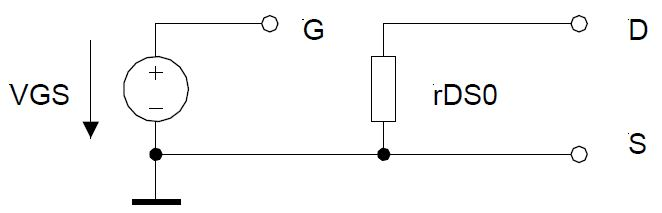
\includegraphics[height=1.5cm]{chapters/Transistoren/images/Ersatzsch_unges}&
	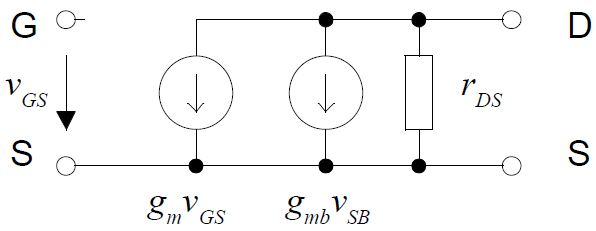
\includegraphics[height=1.6cm]{chapters/Transistoren/images/KS_ges_PI_Bulk}&
	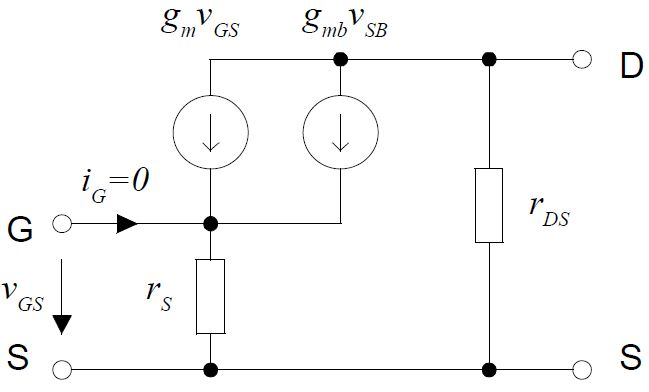
\includegraphics[height=2.2cm]{chapters/Transistoren/images/KS_ges_T_Bulk}&
	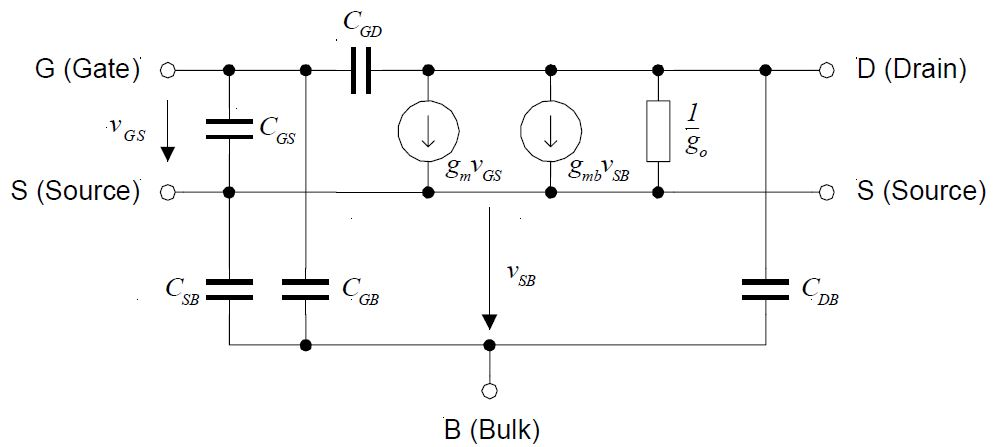
\includegraphics[height=2.2cm]{chapters/Transistoren/images/KS_HF}\\ \hline
\end{tabular}

\subsection{Kleinsignalparameter}
\begin{tabular}{|p{0.2\textwidth}|p{0.35\textwidth}|p{0.35\textwidth}|}
	\hline
	&\textbf{Transistor ungesättigt}&\textbf{Transistor gesättigt}\\ \hline
	weak inversion&Kanalwiderstand bei $V_{DS}=0$:&Kanalwiderstand:\\
	&$r_{DS0}=\frac{dV_{DS}}{dI_D}\vert_{V_{DS}=0} = \frac{\Phi_t}{I_{D0}}$ &$r_{DS}=\frac{1}{g_0}=\frac{dV_{DS}}{dI_D}=\frac{V_A+V_{DS}}{I_D}\approx\frac{V_A}{I_D}$\\
	&Kanalwiderstand bei $V_{DS} = \SI{0}{\volt} \dots V_{DS,sat}$:&\\
	&$r_{DS}=\frac{dV_{DS}}{dI_D}\approx \frac{\Phi_t}{I_D}e^{\frac{V_{DS}}{\Phi_t}}$ (ungenau, kaum benötigt)&\\ \cline{2-3}
	&$g_m$ nicht benötigt&Steilheit\\
	&&$g_m = \frac{dI_D}{V_{GS}}=\frac{I_D}{n_M\Phi_t}$\\ \hline
	strong inversion&Kanalwiderstand bei $V_{DS}=0$:&Kanalwiderstand:\\
	&$r_{DS0}=\frac{dV_{DS}}{dI_D}\vert_{V_{DS}=0}=\frac{1}{\beta(V_{GS}-V_T)\textcolor{gray}{(1+\lambda V_{DS})}}$&$r_{DS}=\frac{1}{g_0}=\frac{dV_{DS}}{dI_D}=\frac{V_A+V_{DS}}{I_D}\approx \frac{V_A}{I_D}$\\
	&Kanalwiderstand bei $V_{DS}=\SI{0}{\volt} \dots V_{DS,sat}$:&\\
	&$r_{DS}=\frac{dV_{DS}}{dI_D}=\frac{1}{\beta[(V_{GS}-V_T)-V_{DS}]\textcolor{gray}{(1+\lambda V_{DS})}}$&\\ \cline{2-3}
	&$g_m$ nicht benötigt&Steilheit (zwei Formeln)\\
	&&$g_m = \frac{dI_D}{V_{GS}}=\beta(V_{GS}-V_T)\textcolor{gray}{(1+\lambda V_{DS})}$\\
	&&$g_m = \frac{dI_D}{V_{GS}}=\sqrt{2I_D\beta\textcolor{gray}{(1+\lambda V_{DS})}}=\frac{2I_D}{V_{GS}-V_T}$\\ 
	$g_{mb}= \frac{dI_D}{V_{SB}}= -g_m(n_m-1)$ wobei &&$n_m=1+\frac{\lambda}{2\sqrt{V_{SB}+\Theta_0}}\approx 1.5$\\      \hline
\end{tabular}

\section{Grundschaltungen mit MOS-Transistoren (Kap. 6)}

\begin{tabular}{|p{0.11\textwidth}|p{0.25\textwidth}|p{0.25\textwidth}|p{0.25\textwidth}|}
	\hline
	&\textbf{Source-Schaltung:}&\textbf{Gate-Schaltung:}&\textbf{Drain-Schaltung:} (Source-Folger)\\
	\textbf{Schema}&
	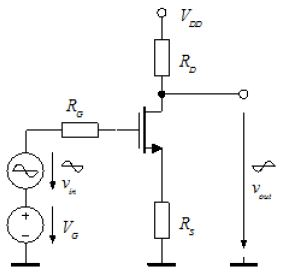
\includegraphics[height=3cm]{chapters/Transistoren/images/GschSource}&
	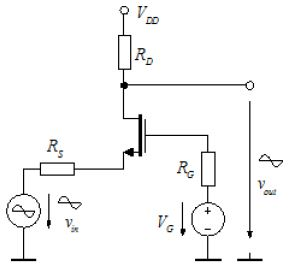
\includegraphics[height=3cm]{chapters/Transistoren/images/GschGate}&
	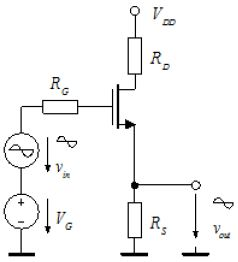
\includegraphics[height=3cm]{chapters/Transistoren/images/GschDrain}\\ \hline
	\textbf{Art}&Invertierender Verstärker&Nichtinvertierender Verstärker&Nichtinvertierender Verstärker\\ \hline
	\textbf{Anwendung}&Verstärkung tiefe bis mittlere Frequenzen&Verstärker hohe Frequenzen (HF-Verstärker)&Spannungsfolger / Impedanzwandler\\ \hline
	\textbf{Eingang}&Gate&Source&Gate\\ \hline
	\textbf{Ausgang}&Drain&Drain&Source\\ \hline
	\textbf{$R_{in}$ / $R_{out}$}&gross/gross&klein/gross&gross/klein\\ \hline
	\textbf{Verstärkung}&\textbf{Bei $1/g_m$,$R_D<<1/g_0$:}&Bei $1/g_m$,$R_D<<1/g_0$:&Bei $R_S$,$R_D<<1/g_0$:\\
	&$a\approx -\frac{R_D}{R_S+\frac{1}{g_m}}$&$a\approx \frac{R_D}{R_S+\frac{1}{g_m}}$&$a\approx \frac{R_S}{R_S+\frac{1}{g_m}}$\\
	&Bei $R_S = 0$: &Bei $R_S = 0$: &Idealer Source-Folger: $A\approx 1$\\
	&$a\approx -g_m(R_D||r_{DS})$&$a\approx g_m(R_D||r_{DS})(1+\frac{g_0}{g_m})$&($1/g_m<<R_S<<1/g_0$)\\ \hline
	\multicolumn{4}{|l|}{$g_m=\frac{1}{r_S}$ \hspace{5mm} $g_0=\frac{1}{r_{DS}}=\frac{I_D}{V_A+V_{DS}}\approx\frac{I_D}{V_A}$ (Näherung für $V_A >> V_{DS}$) \hspace{5mm} $V_A = a_A \cdot L$ ($V_A = \SI{5}{\volt}\dots \SI{100}{\volt}$,Kanallängenabh.)}\\ \hline
\end{tabular}
